\chapter{Introduction}
This document is intended to describe the main steps required for the integration and configuration of RTA-SUM Partial Network Coordinator (PNC). 
\ifnum \DocumentGroup=1
{General guidelines on the common steps and workflow for RTA-SUM integration can be found in \file{SUM Integration - Getting Started}.}
\else
{}
\fi

\section{Definitions and Abbreviations}
\input{generated/tables/definitions.tex}


\section{Module Overview}
RTA-SUM PNC is a software composition located in the Application Layer of the standardized architecture of AUTOSAR, as depicted in Figure \ref{fig:layers}. It implements the following functionalities:
\begin{itemize}
	\item For ECUs that are Activating ECUs, RTA-SUM PNC contains the PN Activation Criteria per the 'Global B PNC Activation Specification'. RTA-SUM PNC is the only SW-C that interfaces with the BSW services to activate and deactivate Partial Networks.
	\item For all ECUs that are Activated ECUs, RTA-SUM PNC interfaces with the BSW services to track the activation status (active or inactive) of the PN.
	\item For all ECUs that are members of any PN, RTA-SUM PNC provides a port that is used to indicate communication capability from RTA-SUM PNC for each SW-C.
	\item Collection of all input signals and input integrity signals (e.g. Rx\_MonitoredSignalAvailability from RTA-SUM SSFM) that are relevant to local Activation Criteria for the PN in which the ECU participates. (Integrity signals apply to both the hardware and communication based signals.)
	\item Collection of all conditional logic related to local activation criteria for the PN in which the ECU activates / deactivates.
	\item Execute a sequence to fulfill the activation of a PN request.
	\item Execute a sequence to fulfill the deactivation of a PN request.
	\item Identify PN mapping to communication channel(s).
\end{itemize}

\newpage

\begin{figure}[htp]
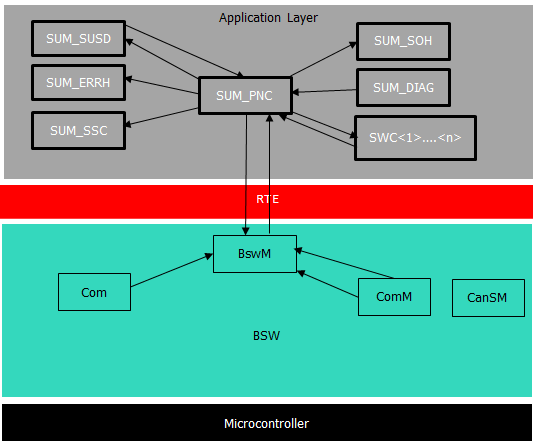
\includegraphics[width=\textwidth]{images/layers.png}
\caption{System layer overview.}
\label{fig:layers}
\end{figure}

\newpage

\section{References}
\input{generated/tables/references.tex}

\section{User Guide Revision History}
\input{generated/tables/rev_history.tex}

